% This is where Assessors will be looking for signs of success and for evidence of thorough and systematic evaluation. Sample output, tables of timings and photographs of workstation screens, oscilloscope traces or circuit boards may be included. Care should be employed to take a professional approach throughout. For example, a graph that does not indicate confidence intervals will generally leave a professional scientist with a negative impression. As with code, voluminous examples of sample output are usually best left to appendices or omitted altogether.

% There are some obvious questions which this chapter will address. How many of the original goals were achieved? Were they proved to have been achieved? Did the program, hardware, or theory really work?

% Assessors are well aware that large programs will very likely include some residual bugs. It should always be possible to demonstrate that a program works in simple cases and it is instructive to demonstrate how close it is to working in a really ambitious case.

% graphs, performance, ablation
% run in mininet
% https://hub.docker.com/r/iwaseyusuke/mininet/
% discuss the implications of the graph
%base on evaluation chapter of papers!

Text here!

\section{Testing methodology}
% describe sofia server
Evaluation was carried out on the computer laboratory's Sofia server (2x Xeon Gold 6230R chips, 768GB RAM). Carrying out experiments on the server should help to minimise interference from other processes on the system.
reiterate somewhere that we use an open loop load generator

\section{Library benchmarks}
\subsection{Cap'n Proto} \label{capnpbenchmark}
I benchmarked the message sending functionality of Cap'n Proto. I did this with an open-loop load generator (which is described in \ref{benchcode}), running each experiment for 10s. I varied the size of messages sent in different tests to replicate the behaviour of the algorithm when sending `batches' of many commands, so a message size of 600 means that the message size is approximately that of a message containing 600 commands.

\begin{figure}[h!]
\centering
\includegraphics[scale=0.75]{dummy_test/throughputgoodput.png}
\caption{Benchmarking of Cap'n Proto server goodput for varying throughputs and message sizes, run for 10s}
\end{figure}

\begin{figure}[h!]
\centering
\includegraphics[scale=0.75]{dummy_test/throughputflatency.png}
\caption{Benchmarking of Cap'n Proto server latencies for varying throughputs and message sizes, run for 10s. Discarded result if goodput was not within 5\% of target throughput.}
\end{figure}

\begin{figure}[h!]
\centering
\includegraphics[scale=0.75]{dummy_test/throughputlost.png}
\caption{Benchmarking of Cap'n Proto server \% of failed requests for varying throughputs and message sizes, run for 10s}
\end{figure}

The figures demonstrate that the framework has a severe drop in performance when sending large messages. For a message size of 600 the goodput goes to zero as the throughput increases, meaning that no messages are being responded to.

[``Fundamentally, there are limitations in the RPC framework that give an upper bound on the performance we can hope to achieve, these limitations are evident in our benchmarking of the Cap'n Proto framework\dots'']

\subsection{Tezos Cryptography} \label{tezosbenchmark}
I profiled the important functions of the library with Jane Street's Core\_bench module [citation needed***]. Core\_bench is a micro-benchmarking library used to estimate the cost of operations in OCaml, it runs the operation many times and uses linear regression to try to reduce the effect of high variance between runs.

\begin{table}[!h]
	\centering
	\begin{tabular}{|l|r|}
	\hline
	Function                 & Time (µs) \\ \hline
	Sign                     & 427.87   \\
	Check                    & 1,171.77 \\
	Aggregate (4 sigs)       & 302.90   \\
	Aggregate check (4 sigs) & 1,179.25 \\
	Aggregate (8 sigs)       & 605.38   \\
	Aggregate check (8 sigs) & 1,180.61 \\ \hline
	\end{tabular}
	\caption{Benchmarking of key functions of the Tezos Cryptography library}
\end{table}
% ┌─────────────┬────────────┬─────────┬──────────┬──────────┬────────────┐
% │ Name        │   Time/Run │ mWd/Run │ mjWd/Run │ Prom/Run │ Percentage │
% ├─────────────┼────────────┼─────────┼──────────┼──────────┼────────────┤
% │ sign        │   427.87us │ 144.00w │          │          │     36.24  │
% │ check       │ 1_171.77us │  75.00w │          │          │     99.25  │
% │ agg_4       │   302.90us │ 484.00w │    0.15w │    0.15w │     25.66  │
% │ agg_check_4 │ 1_179.25us │  75.00w │          │          │     99.88  │
% │ agg_8       │   605.38us │ 944.00w │    0.35w │    0.35w │     51.28  │
% │ agg_check_8 │ 1_180.61us │  75.00w │          │          │    100.00  │
% └─────────────┴────────────┴─────────┴──────────┴──────────┴────────────┘

\section{Benchmarking HotStuff implementation}
\subsection{Batch sizes}
blah blah batch sizes

\begin{figure}[h!]
\centering
\includegraphics[scale=0.75]{batch_size_test/throughputgoodput.png}
\caption{Benchmarking of goodput for varying throughputs and batch sizes, run for 10s}
\end{figure}

\begin{figure}[h!]
\centering
\includegraphics[scale=0.75]{batch_size_test/throughputflatency.png}
\caption{Benchmarking of mean latency while varying throughputs and batch sizes, run for 10s. Discarded result if goodput was not within 5\% of target throughput.}
\end{figure}

\begin{figure}[h!]
\centering
\includegraphics[scale=0.75]{batch_size_test/throughputlost.png}
\caption{Benchmarking of \% requests lost while varying throughputs and batch sizes, run for 10s.}
\end{figure}

\begin{figure}[h!]
\centering
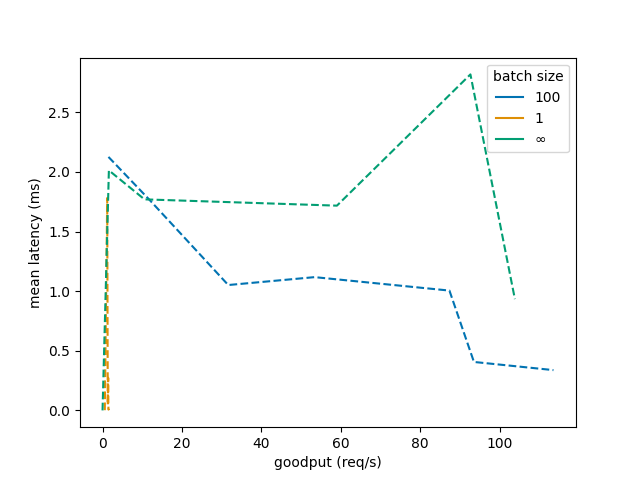
\includegraphics[scale=0.75]{mininet/throughputlatency.png}
\caption{Benchmarking of mean latency while varying throughputs and batch sizes, run for 10s with 100ms network delay.}
\end{figure}

\begin{figure}[h!]
\centering
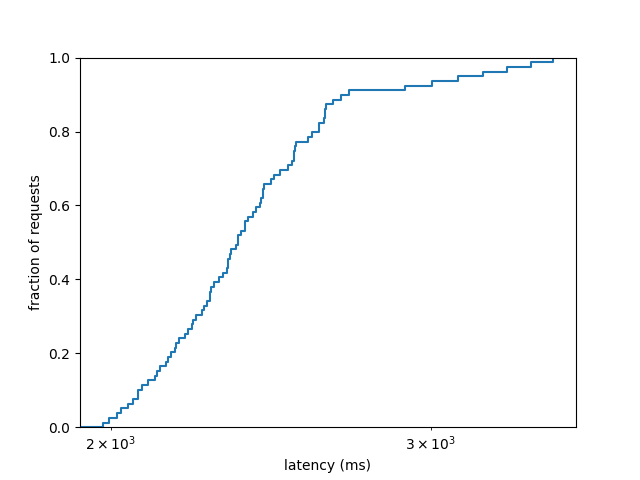
\includegraphics[scale=0.75]{mininet/10tpub_cumlatency.png}
\caption{Cumulative latency plot for experiment with a throughput of 10req/s and unlimited batch size, run for 10s with 100ms network delay.}
\end{figure}

\subsection{Node counts}
blah blah node counts

\begin{figure}[h!]
\centering
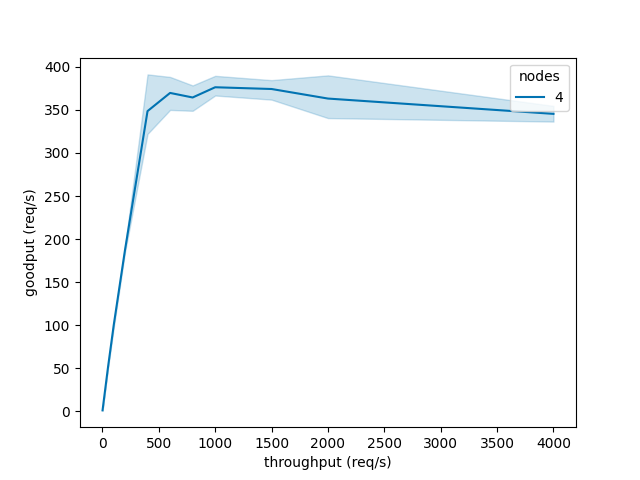
\includegraphics[scale=0.75]{node_count_test/throughputgoodput_nodes.png}
\caption{Benchmarking of goodput for varying throughputs and node counts, run for 10s}
\end{figure}

\begin{figure}[h!]
\centering
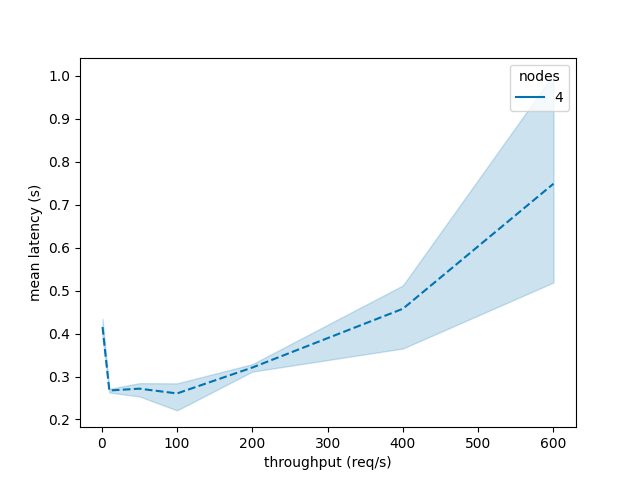
\includegraphics[scale=0.75]{node_count_test/throughputflatency_nodes.png}
\caption{Benchmarking of mean latency while varying throughputs and node counts, run for 10s. Discarded result if goodput was not within 5\% of target throughput.}
\end{figure}

\begin{figure}[h!]
\centering
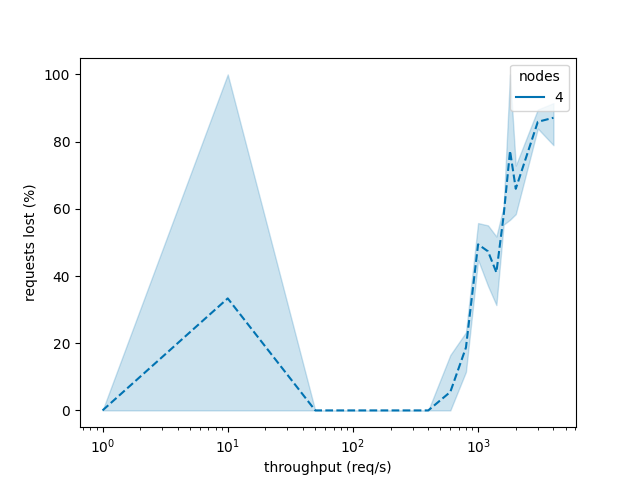
\includegraphics[scale=0.75]{node_count_test/throughputlost_nodes.png}
\caption{Benchmarking of \% requests lost while varying throughputs and node counts, run for 10s.}
\end{figure}

\subsection{Ablation study} \label{ablation}
[``This change improved performance by reducing the amount of time spent waiting in the main loop, the difference is shown in an ablation study'']
blah blah ablation.

Versions:
[turn me into a table!! with caption ``versions'']
\begin{enumerate}
	\item Unchained version
	\item Chained version - node truncation disabled, command filtering disabled
	\item Chained version - node truncation disabled, command filtering enabled
	\item Chained version - node truncation enabled, command filtering disabled
	\item Chained version - node truncation enabled, command filtering enabled
\end{enumerate}

\begin{figure}[h!]
\centering
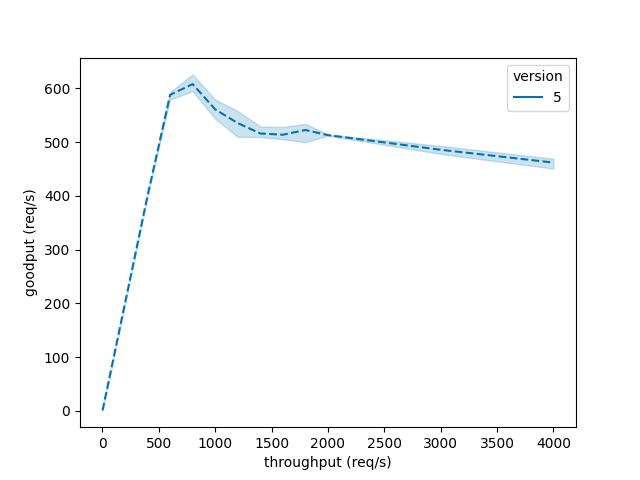
\includegraphics[scale=0.75]{ablation/throughputgoodput_ablation.png}
\caption{Benchmarking of goodput for varying throughputs and implementation versions, run for 10s with 4 nodes unlimited batch size.}
\end{figure}

\begin{figure}[h!]
\centering
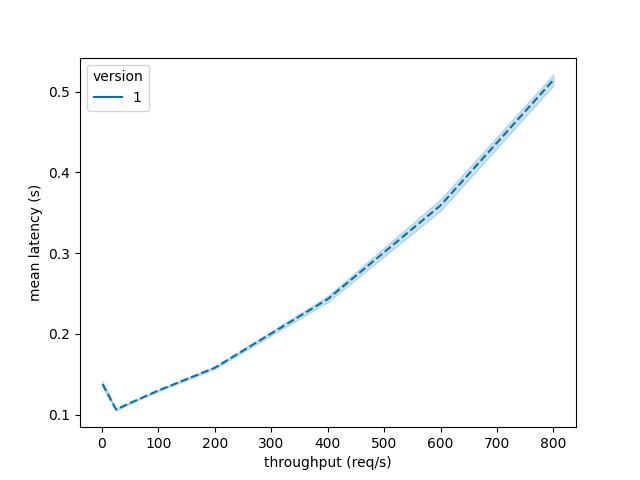
\includegraphics[scale=0.75]{ablation/throughputflatency_ablation.png}
\caption{Benchmarking of mean latency while varying throughputs and implementation versions, run for 10s with 4 nodes unlimited batch size. Discarded result if goodput was not within 5\% of target throughput.}
\end{figure}

\begin{figure}[h!]
\centering
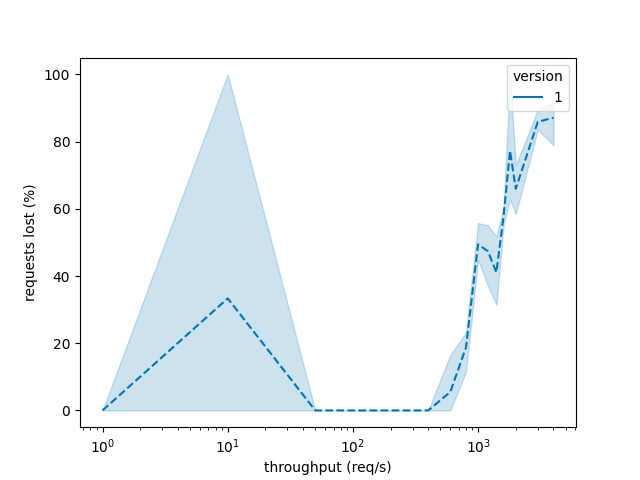
\includegraphics[scale=0.75]{ablation/throughputlost_ablation.png}
\caption{Benchmarking of \% requests lost while varying throughputs and implementation versions, run for 10s with 4 nodes unlimited batch size.}
\end{figure}

\subsection{View change}
\begin{figure}[h!]
\centering
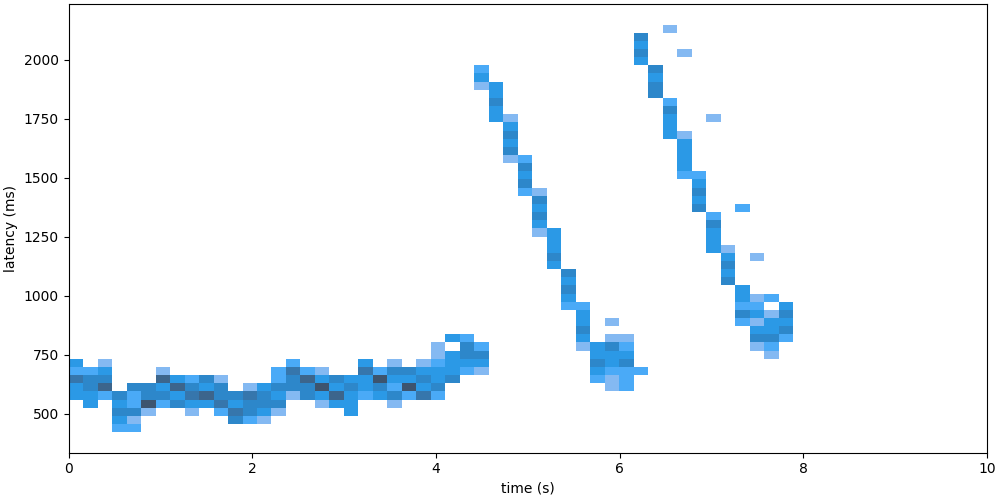
\includegraphics[scale=0.5]{viewchange/test7_100_7_100_timelatencyheatmap.png}
\caption{Heatmap showing distribution of latencies with a node being killed 5s in. Run for 10s with 7 nodes and a batch size of 100.}
\end{figure}
% Clone github.com/cjen1/reckon

% ```
% # This is likely to take a while
% make reckon-mininet

% docker run -it --privileged -e DISPLAY --network host --name reckon-mininet cjen1/reckon:latest bash

% # Set up mininet net with a single switch and 3 nodes
% # drops you into a cli (you can also use python scripting)
% mn --topo single,3

% # observe no delay between nodes
% mininet> h1 ping h2
% mininet> <Ctrl-C>/<Ctrl-D> to exit

% # syntax is `mininet> <node> <command>`
% # I run screens on each node and then attach to those from outside mininet to run the tests in different terminal screens. (Tmux doesn't work correctly afaicr)

% mininet> h1 screen -dmS node_h1 bash

% #Then in another terminal session
% docker exec -it reckon-mininet bash
% screen -r node_h1
% <whatever commands you want to run on that emulated node>

% #Similarly for the other nodes
% ```